\documentclass[addpoints]{exam}
\usepackage[utf8]{inputenc}




\usepackage{pdfsync}
\usepackage{fontspec}
\usepackage[T1]{fontenc}
\usepackage[utf8]{inputenc}
\usepackage{etoolbox}
\usepackage{tikz}
\usepackage{pgfplots}
\usepackage{subfig}
\usepackage{tikzscale} % Scale the figure not the font
\tikzset{
font={\fontsize{5pt}{5}\selectfont}}
\usepackage{tikzscale} % Scale the figure not the font
\usepackage{textpos}
\usepackage{standalone}
\usepackage{color}
\pgfplotsset{tick scale binop=\times}
\usepackage{tikz-dimline}
\usepackage[skins,theorems]{tcolorbox}
\usepackage{animate}


\usepackage{amsmath}
\usepackage{booktabs}
\usepackage{cancel}
\usepackage{caption}
\usepackage{cleveref}
\usepackage{colortbl}
\usepackage{csquotes}
% \usepackage{helvet}
% \usepackage{millennial}
\usepackage{multirow}
\usepackage{listings}
\usepackage{xcolor}

\usepackage{esint} % various fancy integral symbols
\usepackage{outlines}

\usepackage{hyperref}
\hypersetup{
    colorlinks=true,
    linkcolor=blue,
    filecolor=magenta,      
    urlcolor=cyan,
}


\usepackage{physics} % For using the oridnary derivative
\usepackage{siunitx}
\sisetup{per=slash, load=abbr, output-complex-root = j, complex-root-position = before-number, round-mode=figures,round-precision=4}

%% Tikz Libraries
\usetikzlibrary{positioning}
\usetikzlibrary{arrows}
\usetikzlibrary{patterns}
\usetikzlibrary{backgrounds}
\usetikzlibrary{calc}
\usetikzlibrary{decorations.pathreplacing}



\newcommand{\ti}[1]{\tilde{#1}} % spectral representation
\newcommand{\tnsr}[1]{\underline{\underline{#1}}}

% Symbols
\renewcommand{\O}{\omega}  % omega
\newcommand{\E}{\varepsilon}  % epsilon
\renewcommand{\u}{\mu}  % mu
\newcommand{\p}{\rho}  % rho
\newcommand{\x}{\times}  % times
\renewcommand{\inf}{\infty}  % infinity
\newcommand{\infint}{\int\limits_{-\inf}^\inf} % integral by R
\newcommand{\e}{\mathrm{e}} % Straight-up exponential
\renewcommand{\j}{{j}\mkern1mu} % Straight-up exponential
\newcommand{\iu}{\mathrm{i}\mkern1mu}

\newcommand\ddfrac[2]{\frac{\displaystyle #1}{\displaystyle #2}}

\title{High Frequency Communication Systems}
\author{Homework 6 - Two Dimensional FDTD}
\date{Semester 2, 2020/21}

\begin{document}

\maketitle


\begin{questions}
    \pointsinrightmargin 
    \bracketedpoints
\question[3] Modify the code in the notebook and simulate a PEC slab of width  $w = \SI{25}{\mm}$.

\question[2] Create a sinusoidal excitation source $J_z = \sin(n\times\pi/10)$ that lasts in the time duration $n \ge 1$ and $n \le 10$

\question
For the boundary conditions, write down the expressions for the below and show them for the sinsoidal excitation above:
\begin{parts}
    \part[2]
    PEC boundary
    \part[2]
    PMC boundary
    
    \end{parts}


\question[5]

Create a structure as shown in the figure below and find the transmission and reflection of a wave. Use the absorbing boundary conditions and find the transmission at $\SI{10}{\cm}$ distance from the structure on the right.

\begin{figure}[htbp]
    \centering
    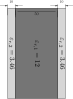
\includegraphics[width=0.4\textwidth]{homework_FDTD_problem3.pdf}
    \caption{Multilayer Structure}
\end{figure}

Note: the thickness units in the simulation are arbitrary. Please go to the next page for submission instructions.

\end{questions}

\section*{Submission Instructions}
Fork the \href{https://github.com/hasantahir/HFCS_lecture}{Github repository}. Create a new cell for each question. For submission, you will have to provide the Github link for where you have deposited the modified repo or give us the \href{https://mybinder.org/}{My Binder} link where we can directly run your notebook.
\end{document}

